\documentclass[9pt,twocolumn,twoside]{styles/osajnl}
\usepackage{fancyvrb}
\journal{i524} 

\title{Triana}

\author{Abhishek Naik}

\affil[1]{School of Informatics and Computing, Bloomington, IN 47408, U.S.A.}

\affil[*]{Corresponding authors: ahnaik@indiana.edu}

\dates{paper-1, \today}

\ociscodes{Triana, Problem Solving Environment, I524}

% replace this with your url in github/gitlab
\doi{\url{https://github.com/absnaik810/sp17-i524/blob/master/paper1/S17-IR-2022/report.pdf}}


\begin{abstract}
Triana is an open source problem solving environment (PSE).  It
provides a powerful data analysis tool alongwith a intuitive visual
interface.  It is mainly used in the areas of signal, text and image
processing. It comes with a set of inbuilt data analysis tools and
also provides easy mechanisms for the integration of custom built
ones.\newline
\end{abstract}

\setboolean{displaycopyright}{true}

\begin{document}

\maketitle

\section{Introduction}

Triana is an open source Problem Solving Environment (PSE) that is
supported with a powerful data analysis tool.  It is predominantly
used for image, text and signal processing; and comes with a host of
different tools for analysis.  Besides, it also provides features for
easy integration of custom analysis tools.  It thus focuses on
supporting services from various environments, like peer-to-peer (P2P)
and Grid.

\section{Features}
Triana has a graphical interactive environment that can be used by the
users to create their applications and specify their behavior
\cite{TrianaDocumentation1}.  In this, it is similar to tools like
draw.io and IBM's Rational Rose that provide the user with a graphical
user interface (GUI) to draw the UML diagrams \cite{DrawIO}
\cite{IBM-Rational-Rose}.  Rational Rose and Draw.io are mainly used
for modeling the control flow diagrams like the class diagram,
sequence diagram, etc., while Triana can be used for modeling generic
flows like an audio processing pipeline.  Thus, while conventional
flows like the sequence diagram can be modeled using Triana, it is
better suited for the creation of generic flows.  The users can model
the work flow using the various units onto the workspace and then
depict the relationship between them with some interconnection.  The
Triana PSE can also be extended to promote discovery of web services,
their composition and decomposition.  A sample Triana GUI image has
been shown in Figure 1.

\begin{figure}[htbp]
  \centering
  \fbox{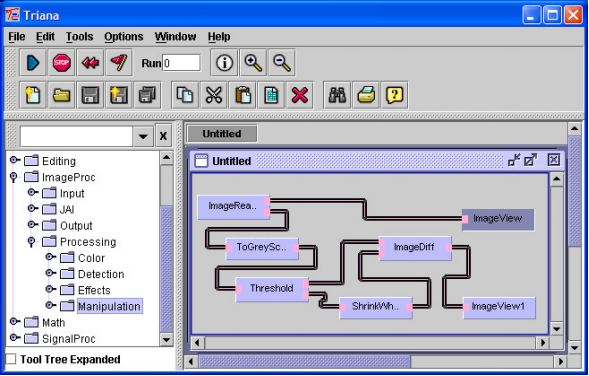
\includegraphics[width=\linewidth]{images/TrianaGUI}}
  \caption{Sample Triana Screen \cite{TrianaDocumentation2}}
\end{figure}

The Triana framework that has been extended with the framework has the 
following set of features: 

\begin{itemize} 

\item Simple creation of the Web services: In case of other frameworks, 
the major challenge is that a composite service cannot be created 
easily. However, by allowing the discovery, composition, invoking and 
publishing of services in an atomic manner, Triana makes this easy. 

\item Execution of services in a distributed fashion: Services can be 
executed on a P2P or Grid middleware using Triana. 

\item 'What-if' analysis: 'What-if' analysis can be easily carried out 
using Triana, by monitoring the different resulting work flows. 

\item Annotation: Triana allows the work flows to be annotated for later 
use. 

\end{itemize}

Triana was originally developed for the GEO600
gravitation project.  In this project, it is still being used for
analysing the gravitational wave signals that emanate from the laser
interferometer based out of Germany \cite{TrianaGEO600}.  Triana uses 
a pluggable architecture, that is it checks the inputs
coming to, and the outputs coming from various units in real time to
perform data-type checking and conformation \cite{TrianaDocumentation2}.  
It can also be used to monitor the work flow and run the executables in standalone mode.
  It has a custom work flow language, although it can
be integrated with others like the Business Process Execution Language
(BPEL) \cite{RMBDP-Book}.  This helps it in analysing large data sets and makes it
particularly important in big data analysis.

\section{Infrastructure}

The Triana infrastructure consists of the
Triana Controlling Service (TCS) that has a Triana Engine, implemented
as a Triana service \cite{TrianaDocumentation2}.  The Triana engines 
are free to carry out the execution either locally or on distributed servers,
as per the implementation policies in force.  Communication in the later case can
be carried out using pipelined work flow distributions.

The Triana Distributed implementation makes use of Triana Group units.
They have the same features of the normal units (like input/output,
etc.) and so they can be connected to the other Triana Units using the
standard connection mechanism.  The tools need to be group so that
they can be distributed; and Triana has two distribution policies -
(a) Parallel: a 'farming-out' mechanism involving no communication between
the hosts; and (b) Pipeline: this involves distributing the group
'vertically'.  Groups can in turn contain groups and each group can in
turn, have its own distribution policy to be followed.  The Triana
distribution mechanisms are based upon the concept of GAT (Grid
Application Toolkit).  The GAT aims to shield the applications from
the implementation details using a standard Application Programming
Interface (GAT-API).  It also provides a set of Grid services for
carrying out tasks such as resource and information management.

Triana is further divided into a set of pluggable components that can 
actively interact with each other. The GUI connects to the engine either 
locally or via a network. Thus, the clients can log in into TCS and view 
the results onto their devices, although the unit in itself might be 
remote. They also have the option to log off and then log in again using 
a different device altogether. In this way, the Triana can be used as a 
monitoring system. Furthermore, there are three ways in which Triana can 
be used, namely: 

\begin{itemize} 

\item Using the GUI on top of an existing application. The various 
interfaces can be used to connect various applications with Triana. 
There are the work flow writers as well as the command writers. 

\item Using the remote control facility of an existing application. The 
Triana facility can be used in exactly the same way as highlighted 
above, but in addition to it, the facility of logging in and off can 
also be leveraged. Here, the scheduling would be implemented by a third 
party system. 

\item Forming various Triana units. This is the best and the most 
preferred way of usage since it becomes very easy to prototype and can 
be easily distributed using the Triana distribution mechanisms. 

\end{itemize} 

Triana has a pluggable architecture that can be extended using the 
Triana GUI as a front end to some standalone application. This can be 
carried out using the inbuilt task-graph or command writers. Custom 
writers can also be used. Similarly, it can also be extended by 
implementing the same set of interfaces that the Triana Control Service 
includes. Another way of extension is by implementing custom Triana 
units to achieve the desired functionality. This would require the 
building of a number of Triana components and their seamless integration 
with inbuilt components.

GAT provides simple communication mechanism with Triana. The calls are 
independent of the GAT middleware binding. This decoupling enables easy 
porting of Triana on different Grid middleware without any modification 
to the core Triana code. Furthermore, the Triana project is concurrently 
being developed with the GridLab project, that is developing the GridLab 
GAT. The Triana is precisely being used as a test application to develop 
requirements from the GridLab GAT. A prototype GAT API called the GAP 
Interface (Grid Application Prototype Interface) has been developed. 
This Interface is basically used for communicating with the remote 
servers, which was one of the main functionalities to be developed as a 
part of the GridLab GAT. JXTA currently has GAP interface bindings. 

The GAP interface bindings implement the basic GAP functionality,
which is locating and communicating the JXTA services. Such a service
has two input nodes and may have multiple output nodes - either zero,
one or more. The input and the output nodes are delegated as the JXTA
pipes and a virtual communication channel is established between
them. This virtual communication channel adapts a particular
communication protocol depending upon the current operating
environment. The relationship between Triana and GAP is shown in
Figure 2.

\begin{figure}[htbp]
  \centering
  \fbox{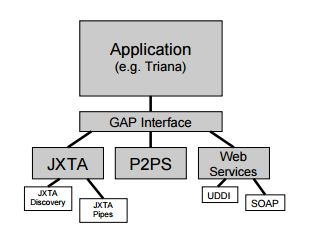
\includegraphics[width=\linewidth]{images/TrianaGAPRelationship}}
  \caption{Relationship between Triana and GAP \cite{TrianaDocumentation1}}
\end{figure}

\section{Projects}

Triana has been involved in a lot of projects (including some Big Data projects) 
like the Data-Mining Grid, 
Scalable Robust Self-organizing Sensor Network Project (SRSS) and 
SHaring Interoperable Work flows for large-scale
scientific simulations on Available DCIs (SHIWA), etc \cite{Triana-projects} 
\cite{Triana-Data-Mining-Grid} \cite{Triana-SRSS} \cite{Triana-SHIWA} .  As a part of
the Data-Mining Grid, Triana was predominantly used to model and then
manage the planning, development and the execution of data-mining work
flows in grid computing environments.  The SRSS
project is carrying out a research about the various communication
protocols that can be leveraged in distributed and self-organizing
networks; and they are using Triana's P2P binding to simulate various
P2P networks \cite{Triana-SRSS}.  The European project, SHIWA, mainly focuses on the
interoperability of myriad European Work flow Systems and has been
intrinsically integrated with Triana to create SHIWA bundles \cite{Triana-SHIWA}.  
Other than these, Triana is also being actively used
in some other projects like EDGI, TRIACS, EDGES, WHIP (Work flows
Hosted In Portals), DART (Distributed Audio Retrieval using Triana),
GridOneD, GEO600, BiodiversityWorld, DIPSO, GEMMS, etc. many of which
are related to Big Data.

Triana was released as an open source project on 30th May 2003. It 
included two GAT bindings - one that was implemented as the JXTA and the 
other as the Java socket based on the P2P mechanism (P2PS). How to run 
Triana, as JXTA or as a Java socket based on P2P mechanism is upto the 
user and the choice he makes at the system start.

\section{Conclusion}

Thus, to conclude, we presented Triana and the Triana PSE.  We focused
on the Triana infrastructure as well as its distributed
implementation.  We also presented some Big Data projects that used
Triana for their development.

% Bibliography

\bibliography{references}

\end{document}
